\chapter{Preprocessamento}\label{pre}


\subsection{Mapa de Pernambuco com as Rodovias Federais em destaque}

\begin{figure}[ht]
	\centering
	\caption{Mapa rodoviário de Pernambuco}
	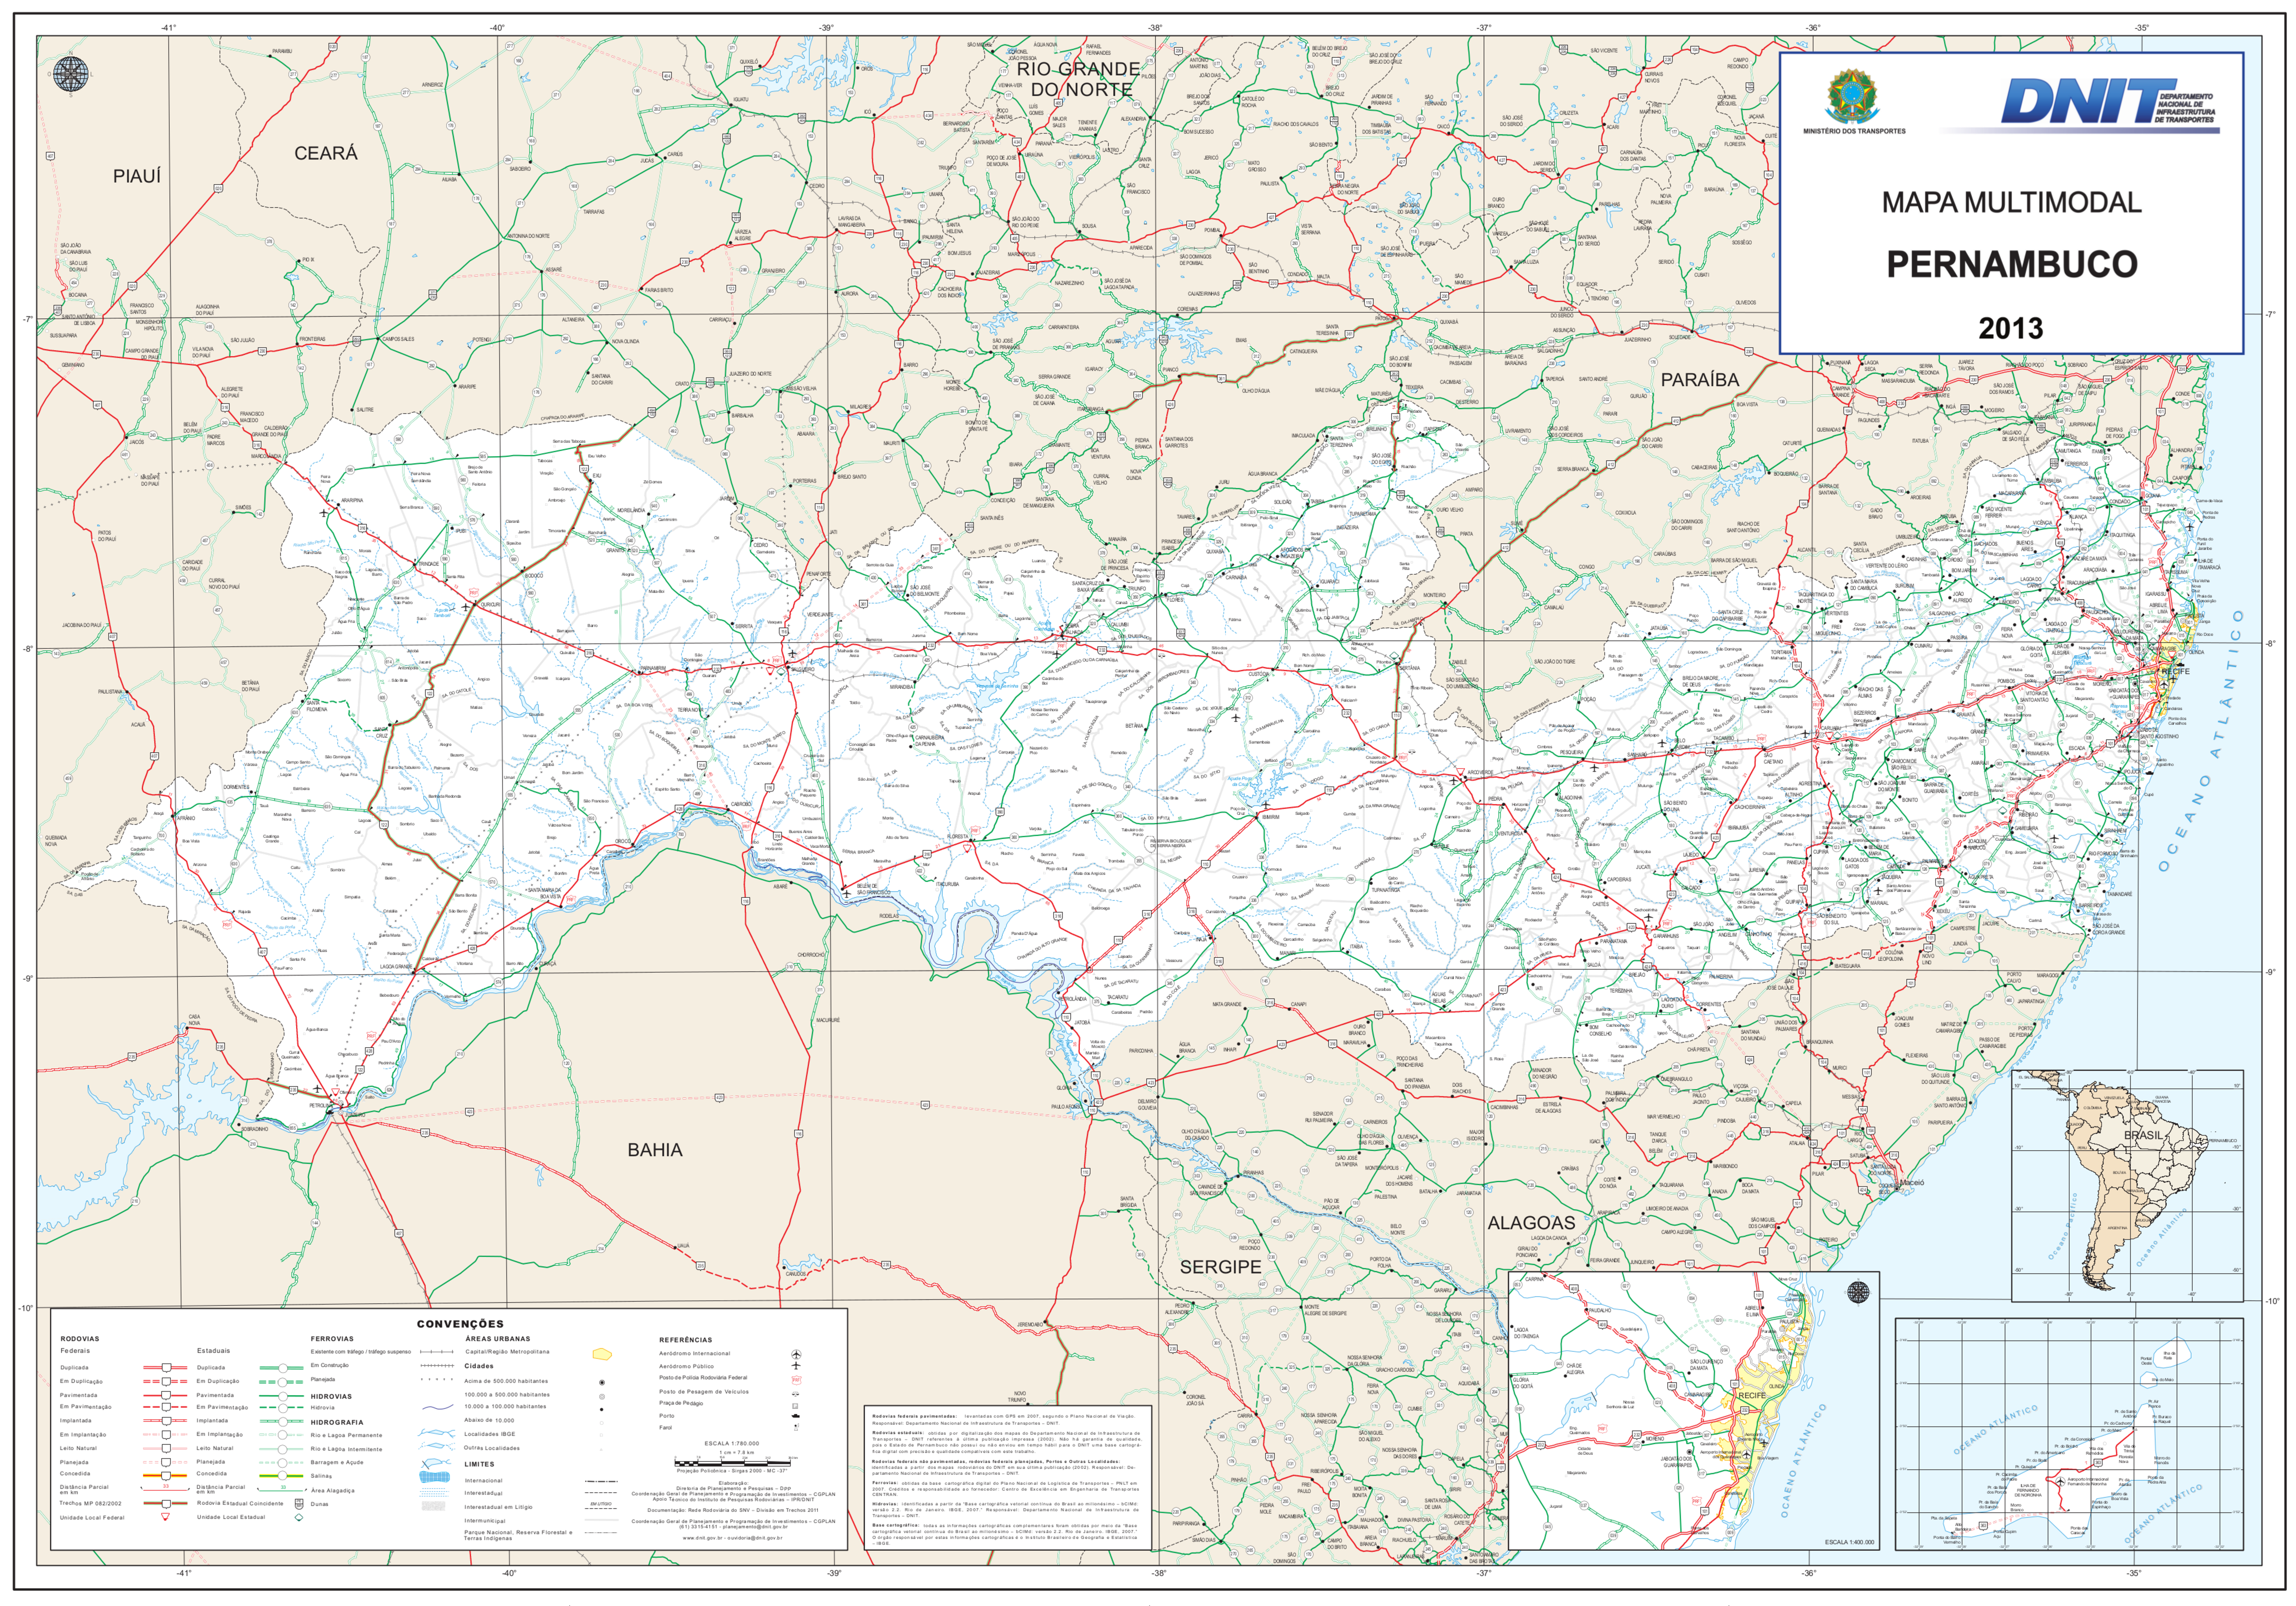
\includegraphics[width=150mm, height=110mm]{Figuras/Anexos/Mapa-pe.pdf}\\
	\tiny Fonte: DNIT
\end{figure}


\section{Coleta e Preprocessamento dos dados da PRF}\label{intro:Anexo}


As informações para suprir nosso modelo preditivo estão disponíveis na Internet, em sua maioria são Dados Governamentais Abertos, tais como os dados
da:
\begin{itemize}
	\item PRF (1) $ https://www.prf.gov.br/portal/dados-abertos/acidentes $
	\item PRF (2) $ http://dados.gov.br/dataset?tags=SIGER$
	\item INPE $ http://www.inpe.br/dados_abertos/ $ 
	\item IBGE $ http://dados.gov.br/dataset?tags=IBGE $
\end{itemize}

Isto são iniciativas governamentais para fomentar a participação popular, dentro outros motivos, essas informações são também 
conhecidas como \textit{open data} \cite{DadosGoverno}. 
Contudo os dados referentes à PRF e ao BPRv, para esta pesquisa, foram cedidos pelos respectivos 
órgãos governamentais (ver autorizações para cessão dos dados da PRF e do BPRv e um 'preview das planilhas) já em formato CSV (ver Figura A.2) para serem utilizados exclusivamente nesta pesquisa. 
Isso possibilitou ganho qualitativo nos dados evitando 
passar pelos transtornos como descreve Costa (2015) quando coletou os dados diretamente da Internet.\cite{Costa2015} 
As bases de dados do INPE e do base de dados do IBGE apresentaram boa qualidade, ou seja: poucos dados ausentes ``missing data'' e consistência (banco de dados relacionais) o que justificou serem serem coletados diretamente da Internet.

Originalmente os dados provenientes da PRF continham 85.209 instâncias, 27 atributos, dentre eles: Km, Latitude, Longitude, Condições da Pista, Causa do Acidente, Município, Data, Hora, Tipo de Veículo, Quantidade de Mortos, Quantidade de Feridos Graves, dentre outros descritos na Tabela A.1


\begin{figure}[ht!]
\centering
\caption{Planilha PRF aberta no Knime}
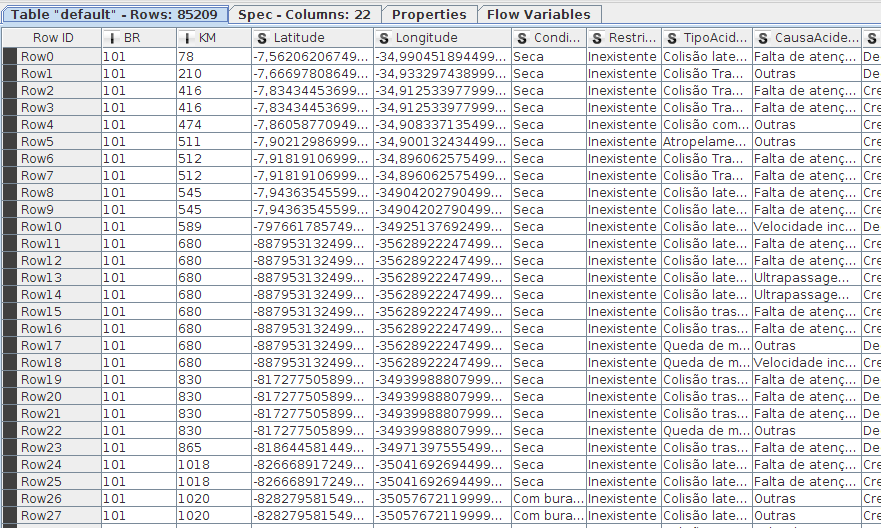
\includegraphics[width=0.9\linewidth]{Figuras/Anexos/PlanilhaPRF.png}
\label{fig:PreviaPlanilhaPRF}\\
\tiny Fonte: PRF/PE
\end{figure}

Como pode ser visto na Figura A.2 os dados vêm separados por vírgula (formato CSV), repletos de dados ausentes (faltas de dados ou ``missing data''). Alguns dados vêm sem as aspas, outros faltando vígula separadora. Por se tratar de 85.000 regitros (dados originais da PRF/PE) é uma trarefa inumana para se verificar visualmente, necessitando portanto de ferramentas especiais. As planilhas eletrônicas como MS Excel ou LibreOffice não deram conta de exibir os dados. Foi escolhido portanto Knime, para visualizar e tratar inicalmente os dados e posteriormente o R. Com os dados já tratados foram inseridos em no MySQL (SGBD) com as tabelas desnormalizadas, formando uma tabela única (ou tabelão, jargão da área de Ciências dos Dados).

%\pagebreak

%%---------------------------------------------------------------------------------------------------

A tabela A.1 representa as variáveis coletadas da base de dados da PRF/PE exibidas na Figura A.2.

\begin{table}[htbp!]
 \centering
  \caption{Variáveis originais da base de acidentes} 
  \begin{tabular}{r|l} \hline
   Ano & Ano da ocorrência do acidente\\
   Mês & Mês de ocorrência do acidente\\
   Num & Número do mês do acidente ex: 1 = Janeiro \\
   KM & Numeração do quilômetro \\
   BR & Numeração da Br\\
   Latitude & Latitude da ocorrência \\
   Longitude & Longitude da ocorrência \\
   Condição Pista & Condição da pista: seca, molhado, ... \\
   Restrição de Visibilidade & Restrição de visibilidade: inexistente, neblina, .., outros \\
   Tipo Acidente & Tipo de Acidente: atropelamento, colisão lateral,..\\
   Cauda Acidente & A possível causa do acidente: Falta de atenção, ... \\
   Sentido Via & Sentido da via: crescente, decrescente \\
   Traçado Via & Tipo de traçado da via: reta, curva, cruzamento, ... \\
   Município  & Localidade onde ocorreu \\
   Tipo veículo & Tipo de veículo envolvido no acidente \\
   Data Inversa & Data do acidente no formato dd/mm/aa \\
   Horário & Hora que ocorreu o acidente no formato hh/mm/ss \\
   Qtd Feridos Graves & Quantidade de feridos graves envolvidos \\
   Qtd Feridos Leves & Quantidade de feridos leves envolvidos\\
   Qtd Ilesos & Quantidade de ilesos envolvidos\\
   Qtd Mortos & Quantidade de mortos envolvidos \\
   Qtd Pessoas & Quantidade de pessoas envolvidos \\
   Qtd Veículos & Quantidade de veículos envolvidos\\
   Qtd Acidentes Graves & Quantidade de acidentes graves \\
   Qtd Ocorrências & Quantidade de ocorrências \\
  \end{tabular}
\end{table}


Na Tabela A.2 apresenta as variáveis originais da base de dados da PRF com interdições das vias 
(somente interdições que paralisaram as BRs, não contém acidentes, exemplo: passeatas, protestos) 

\begin{table}[htbp]
 \centering
  \caption{Variáveis originais da base de interdições}
  
  \begin{tabular}{r|l} \hline
   Comunicação & Código do agente que comunicou o incidente \\
   Data Hora & Data hora no formato dd/mm/aa mm:ss \\
   BR & Numeração da Br do incidente\\
   KM & Numeração do quilômetro do incidente\\
   Trecho  & Local onde ocorreu o incidente \\
  \end{tabular}
\end{table}


\pagebreak

%%----------------------------------------------------------------------------------------------------

\section{Preprocessamento das Bases Históricas}\label{intro:Anexo}

\begin{figure}[ht]
  \centering
    \caption{Etapa 1  -- Coleta e união das bases históricas de acidentes e interdições da Polícia Rodoviária Federal - PE, entre 2007 a 2015}
    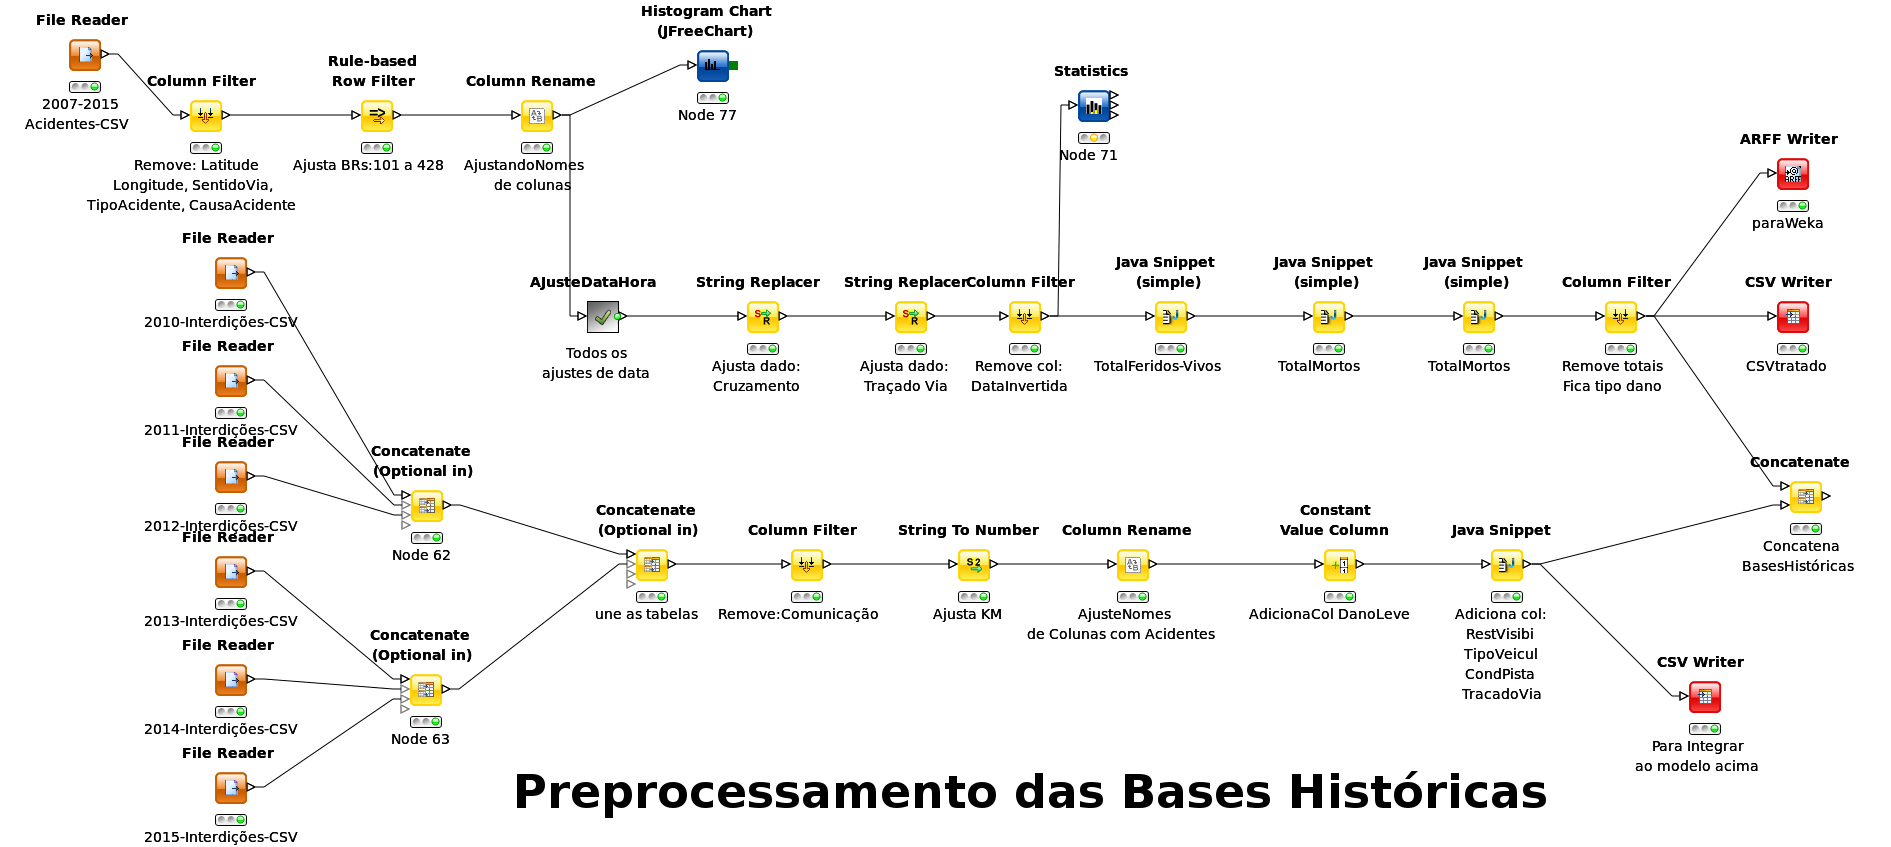
\includegraphics[width=165mm, height=100mm]{Figuras/Cronograma/BasesHistoricas.png}
\end{figure}

A Figura A.3 representa a imagem do ``Workflow'' construído na ferramenta Knime \cite{Knime2}.
Esta ferramenta permite ter uma boa visualização dos dados e tratá-los com ferramentas de programação, aceitando as linguagens Java, Python e R (nossa preferência), através de conexões que são disponibilizadas pela ``framework''.

Os itens da Figura A.3 são:
\begin{itemize}
	\item File Reader: Elemento que carrega dados no formato CSV;
	\item Column Filter: Elemento que permite tratar colunas nas tabelas carregadas;
	\item Rule-base Row Filter: Elemento que permite tratar linhas nas tabelas carregadas;
	\item Columns Rename: Elemento que permite renomar colunas;
	\item Concatenate(optiona in): Elemento que permite concatenar bases de dados diferentes;
	\item String Replacer: Elemento que permite alterar/limpar algum 'lixo' nos dados;
	\item Java Snippet: Elemento que permite utilizar a linguagem Java
	\item ARFF Writer: Elemento que permite gerar output para a ferramente Weka;
	\item CSV Writer:  Elemento que permite gerar output tipo CSV para entrada no R (ou planilhas eletônicas)
	\item Itens em azul são para visualização gráfica dos outputs do workflow
\end{itemize}



\pagebreak



A Figura A.4 representa a sequência de tarefas para tratar os dados provenientes do Twitter. Para isso é preciso ter uma conta no Twitter (http://twitter.com) e registrar  um aplicativo, em seguida os dados são liberados.
\begin{figure}[ht!]
	\centering
\caption{Sequência para tratamento dos dados das Redes Sociais}
	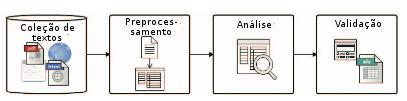
\includegraphics[width=0.7\linewidth]{Figuras/Twitter/prepocesTextos}
	\label{fig:workflow Twitter}
\end{figure}

O ``Workflow'' da figura A.5 é semelhante ao apresentado na Figura A.3, pois importante visualisar os dados e são poucas as ferramentas que permitiram carregar 85.000 registros para tratá-los posteriormente. Na Figura A.5 o elemento ``Twiter API Connection'' permite entrar com os dados ``API Key'' e ``API token'' fornecidos pelo Twitter e que darão acesso aos dados. Os elementos restantes do ``Workflow'' da Figura A.5 são semelhantes aos da Figura A.3.


\begin{figure}[ht!]
\centering
\caption{WorkFlow do Twitter}
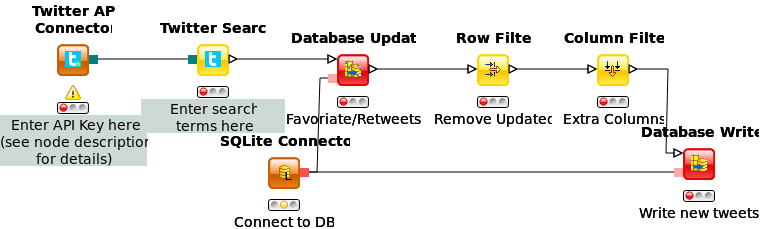
\includegraphics[width=0.7\linewidth]{Figuras/Twitter/workflow}
\label{fig:workflow Twitter no Knime}
\end{figure}

A ferramenta Knime \cite{Knime} foi essencial para essa tarefa de visualização e algum tipo de tratamento nos dados, em especial o tratamento com as datas. Os dados, de uma maneira em geral podem ser tratados no Knime, no R ou no MySQL, contudo achamos mais simples e eficaz utilizar o que cada ferramenta tem de melhor. O MySql para fazer uma análise nos dados, o Knime para visualizá-los e o R \cite{R-cran} para fazer ajustes finais e estatísticas sobre os dados com mais rapidez e transparência.
No Weka \cite{Weka}, com os dados já tratados e limpos foram rodados os algoritmos de I.A.
Estíma-se que 80\% do tempo total da pesquisa foi para tratar os dados.

\pagebreak

Os dados originais do Twitter são conseguidos após preencimento de uma série de requisitos burocráticos e de segurança.
Na ferramente R são preenchidos uma sequência de instruções (credenciais) para se ter acesso aos dados:\\

library(twitteR)\\
$ requestURL = "https://api.twitter.com/oauth/request_token" $\\
$ accessURL = "https://api.twitter.com/oauth/access_token" $\\
$ authURL = "https://api.twitter.com/oauth/authorize" $\\
$ consumer_key = "wtJa6ADnYJM5qCW8ecK---" $\\
$ consumer_secret = "NRKfmkMg06hH30RjVvocvXt814uTEMoLomZp" $\\
$ access_token = "528603134-F4XrgrN8v5jwzxEvxeHIKjyMxajcl" $\\
$ access_secret = "GALsD4zAoopfgLrpBPR4apboUsN6tc0bMo3pL" $\\
$$ setup_twitter_oauth(consumer_key, consumer_secret, access_token, access_secret) $$\\

Após passar essas credenciais o Twitter libera os dados que estão demonstrados na figura A.6, visualizado no LibreOffice.

\begin{figure}[ht!]
	\centering
	\caption{Dados originais do Twitter}
	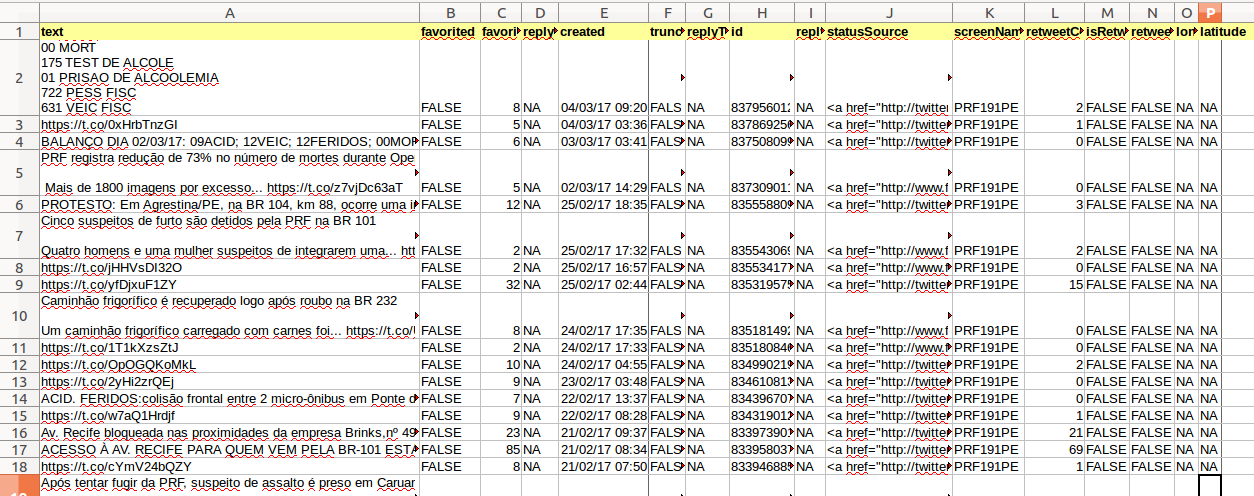
\includegraphics[width=0.9\linewidth]{Figuras/Anexos/tweetPRF}
	\label{fig:workflow Twitter}
\end{figure}

Curiosidades sobre os dados do Twitter utilizados nesta pesquisa:
\begin{itemize}
	\item Dados de 2017 -- 2014 --- canal @PRF191PE
	\item 2864 Instâncias -- 16 Atributos
	\item Dentre eles: 'text, 'favorited', 'favoriteConunt', 'created', 'ID', 'statusSource', 'screenName', 'retweetCount',
	\item 'isRetweet', 'retweeted', dentre outros.		
\end{itemize}

A mineração sobre dados textuais foi feira a partir da variável ``text''. As variáveis ``favorited'', ``retweeted'' dentre outras foram utilizadas para gerar os grafos, ver Figura 2.11.

As Figuras A.7 a A.8 são referentes aos documentos de autorização para liberação dos dados provenientes da PRF e do BPRv.
Os dados do BPRv foram descartados a priori, pois, o modelo proposto, com a solução incluindo somente as BRs atendia. Um trabalho continuado poderia incluir esses novos dados para otimizar o modelo preditivo. A Figura A.9 contém dados da evolução da frota de veículos em Pernambuco. Os dados de 2007 a 2015 serviram para normalizar as Martrizes de Acidentes.


\pagebreak

\begin{figure}[ht!]
	\centering
		\caption{Documento liberação dos dados PRF}
		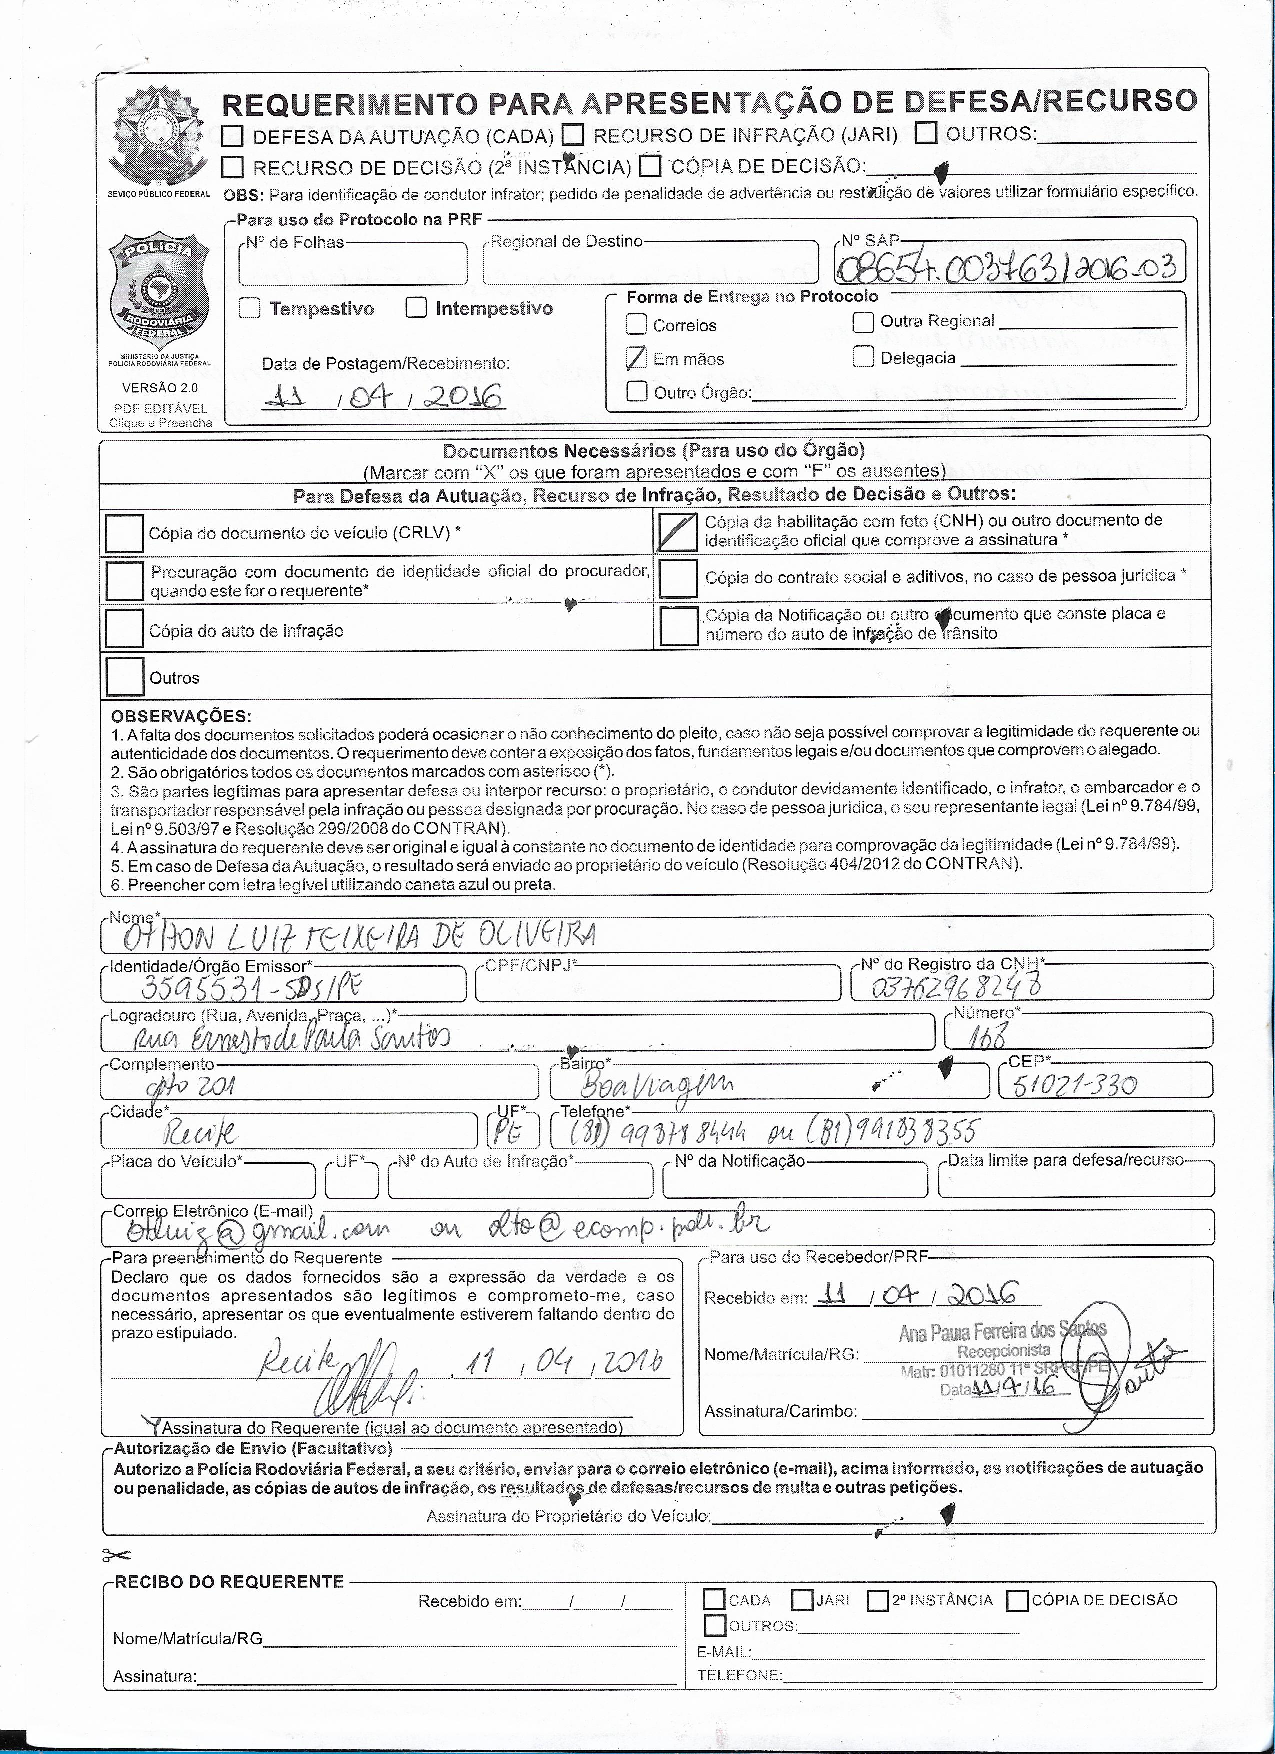
\includegraphics[scale=0.30]{Figuras/Anexos/A1-PRFDadospg_001.pdf}
		\qquad \quad \quad
		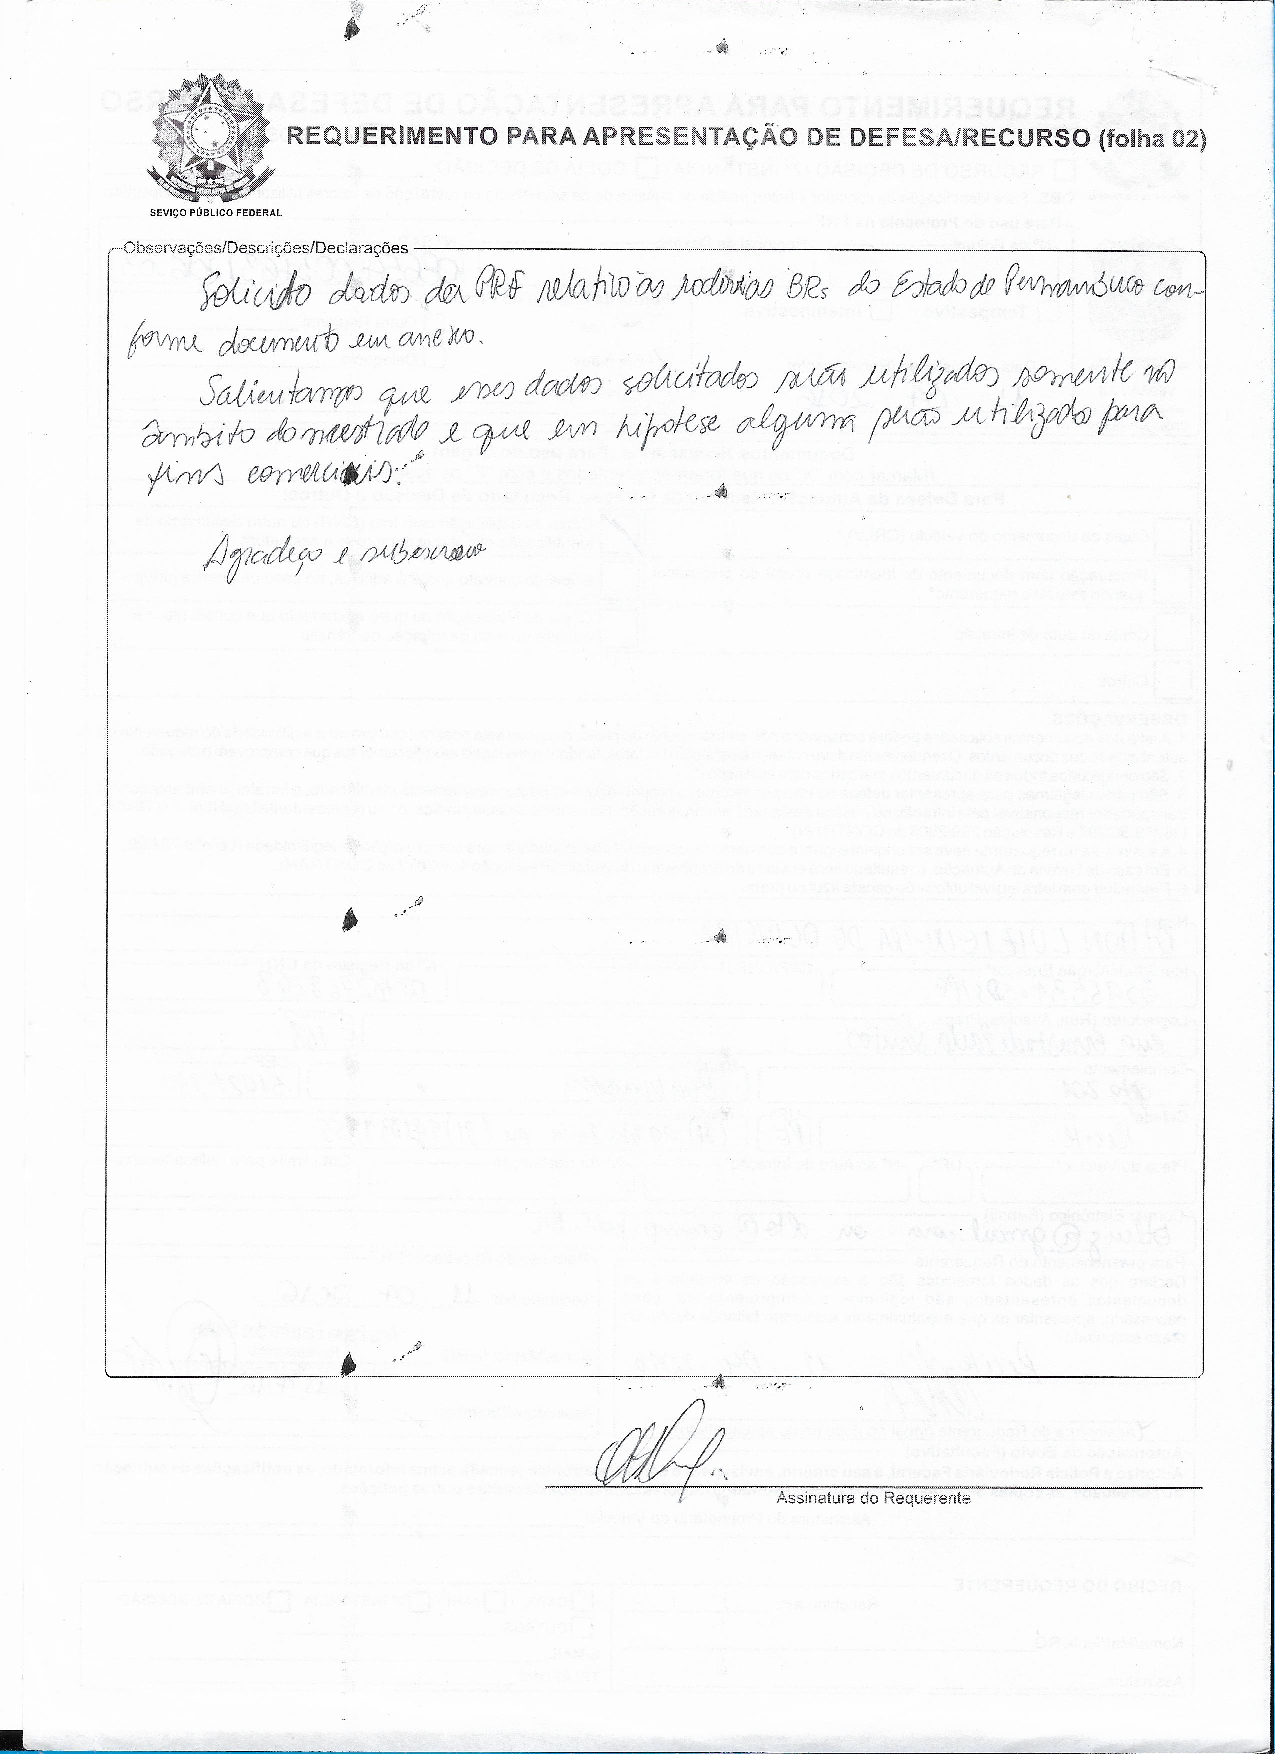
\includegraphics[scale=0.30]{Figuras/Anexos/A1-PRFDadospg_002.pdf}
		\qquad \quad \quad
		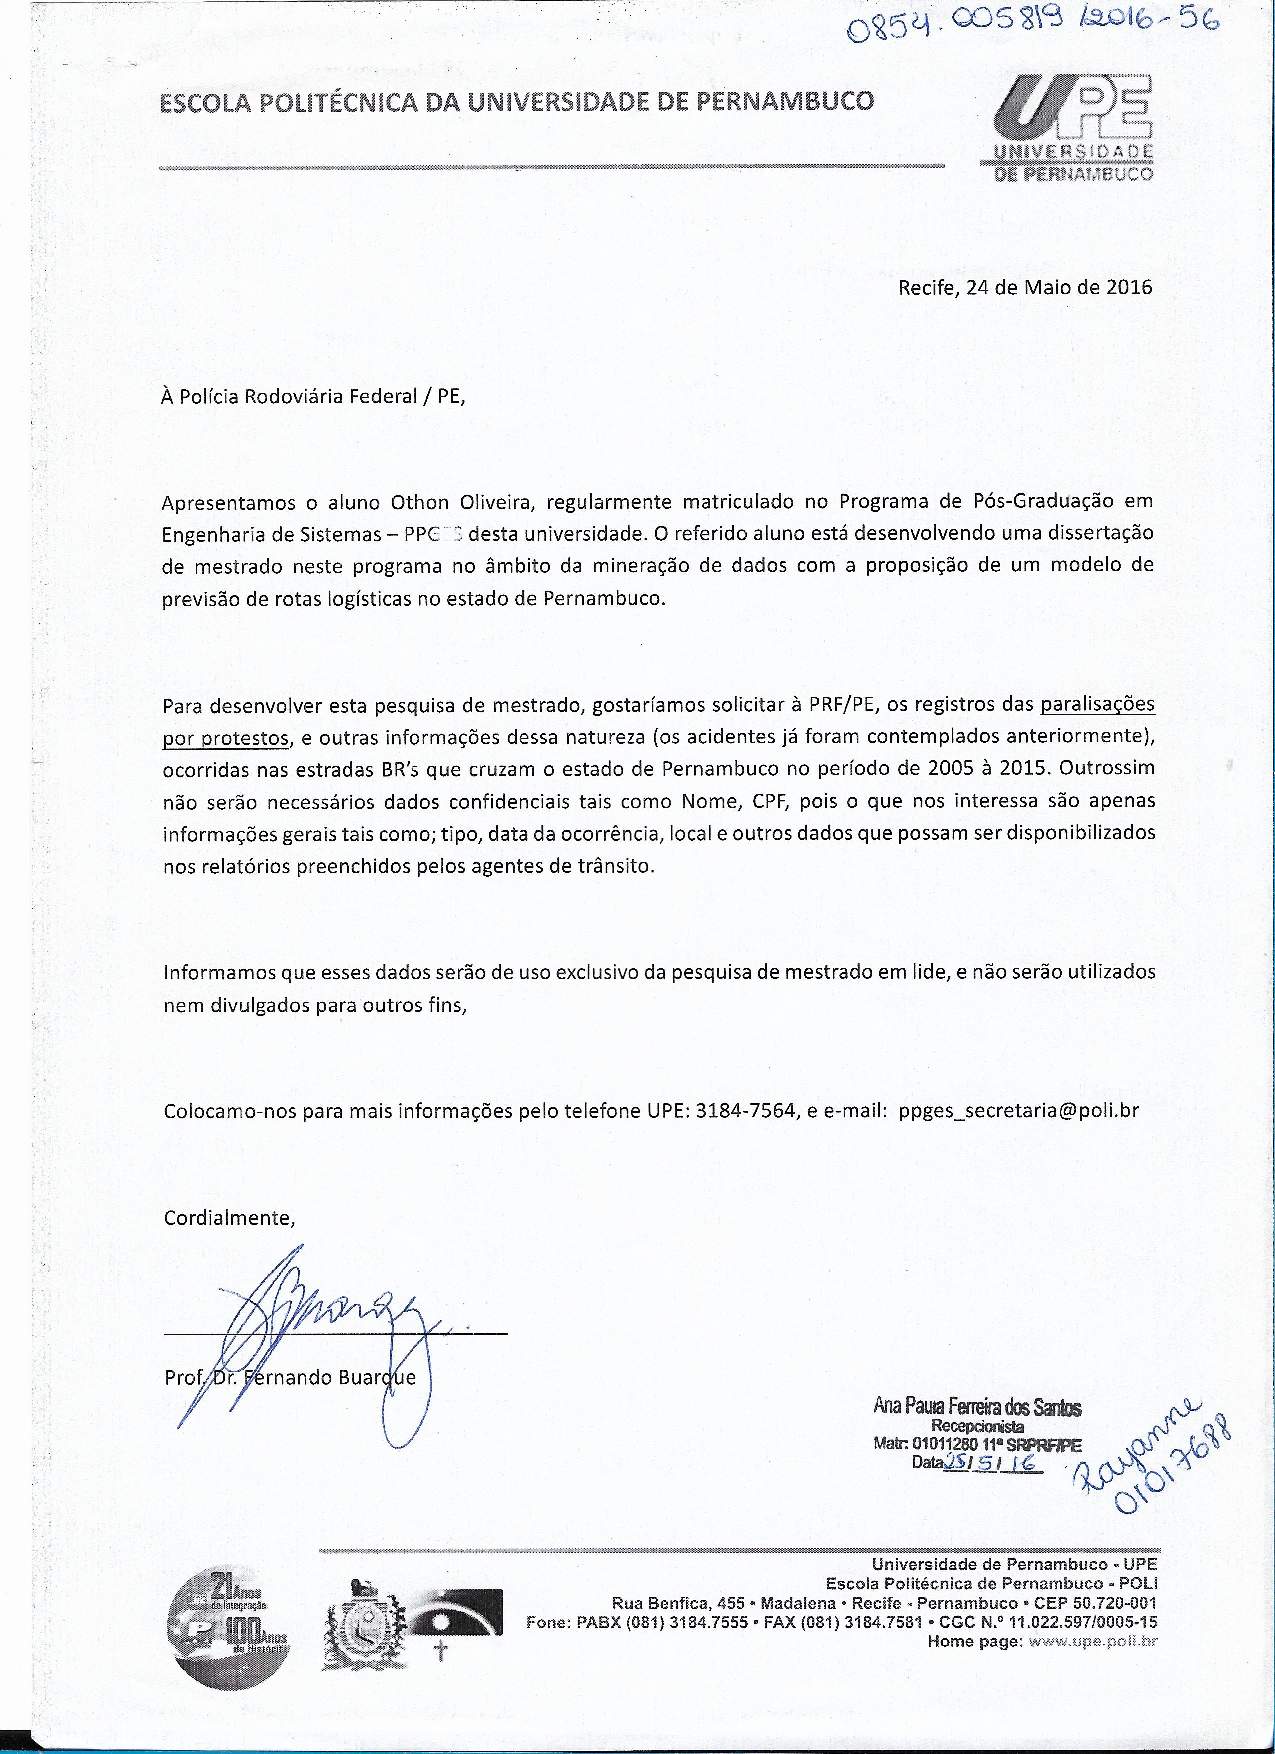
\includegraphics[scale=0.30]{Figuras/Anexos/A1-PRFDadospg_003.pdf}
		\qquad \quad \quad
		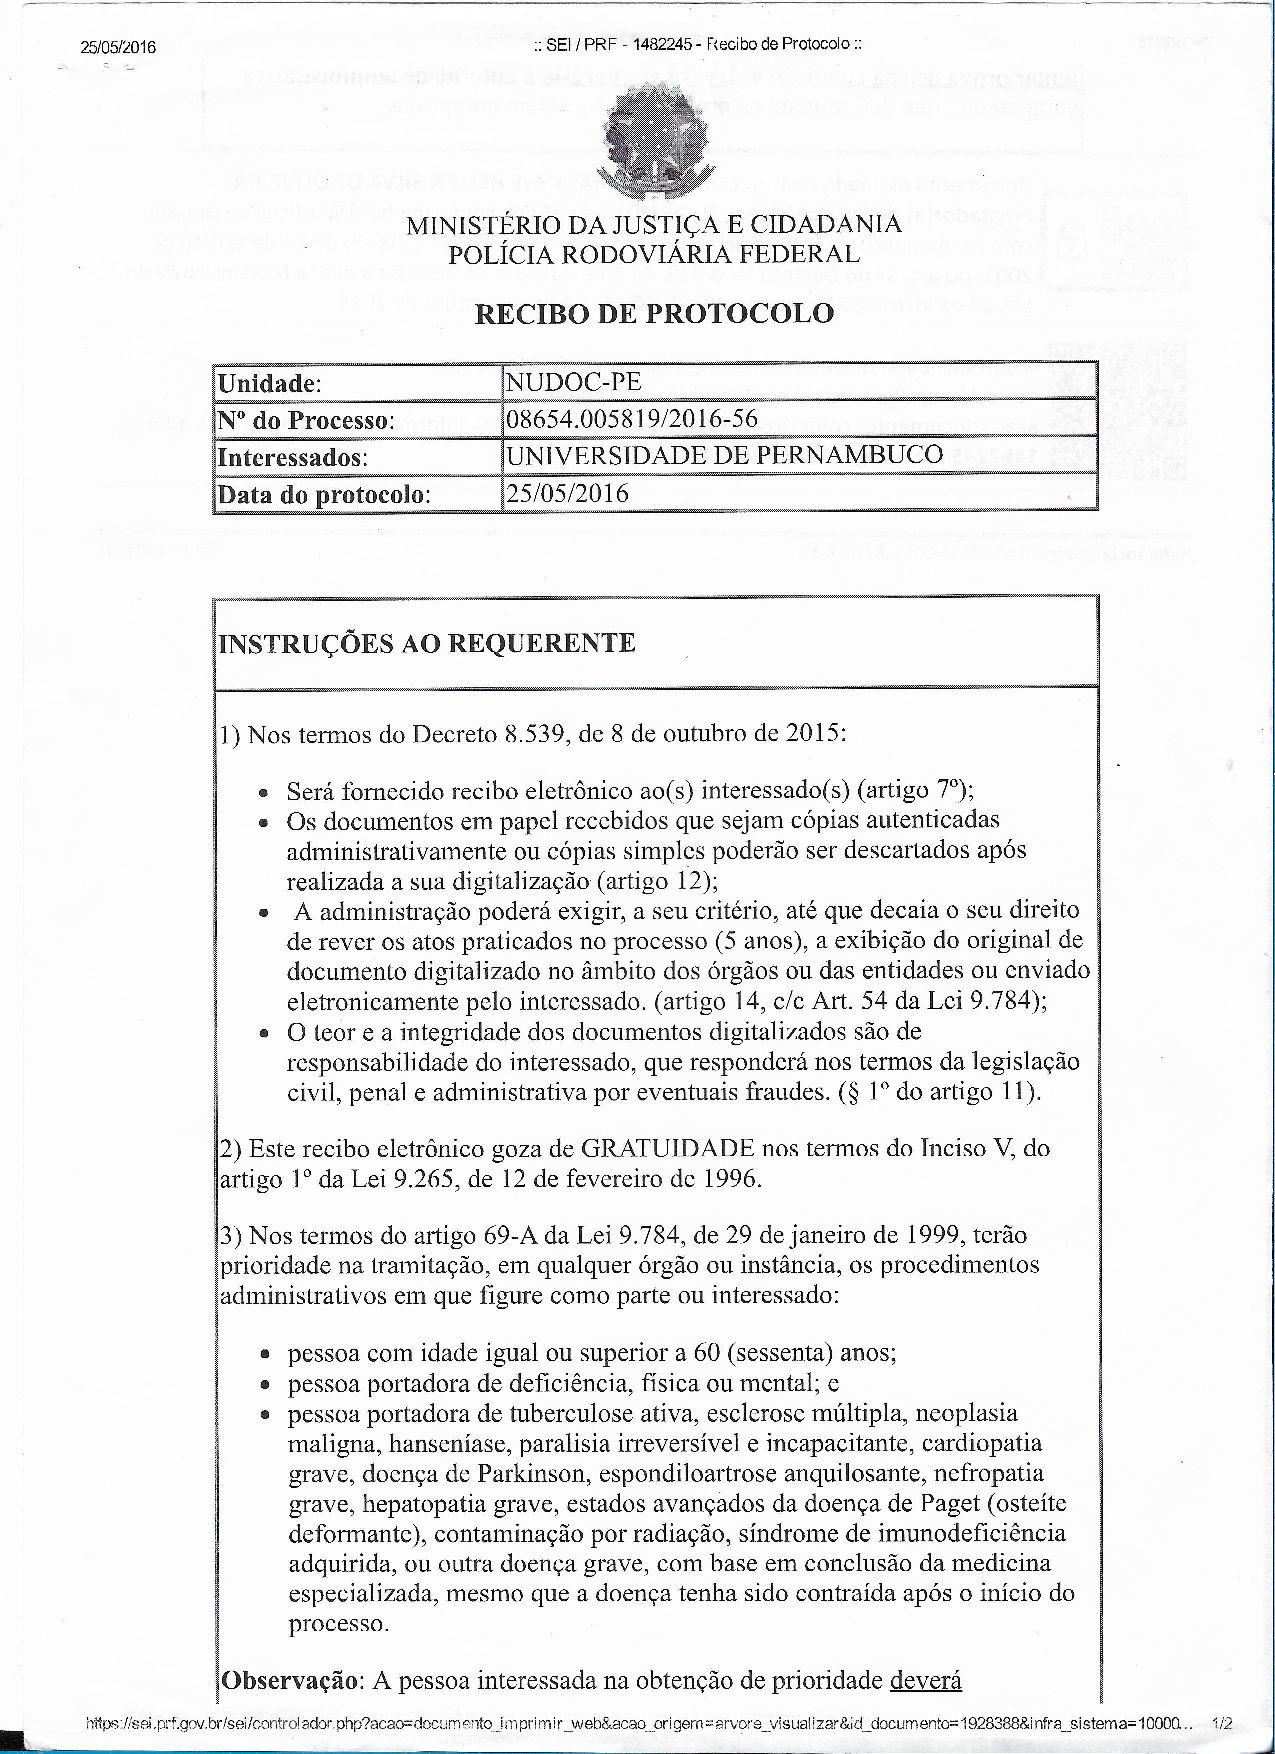
\includegraphics[scale=0.30]{Figuras/Anexos/A1-PRFDadospg_004.pdf}
		\qquad \quad \quad
		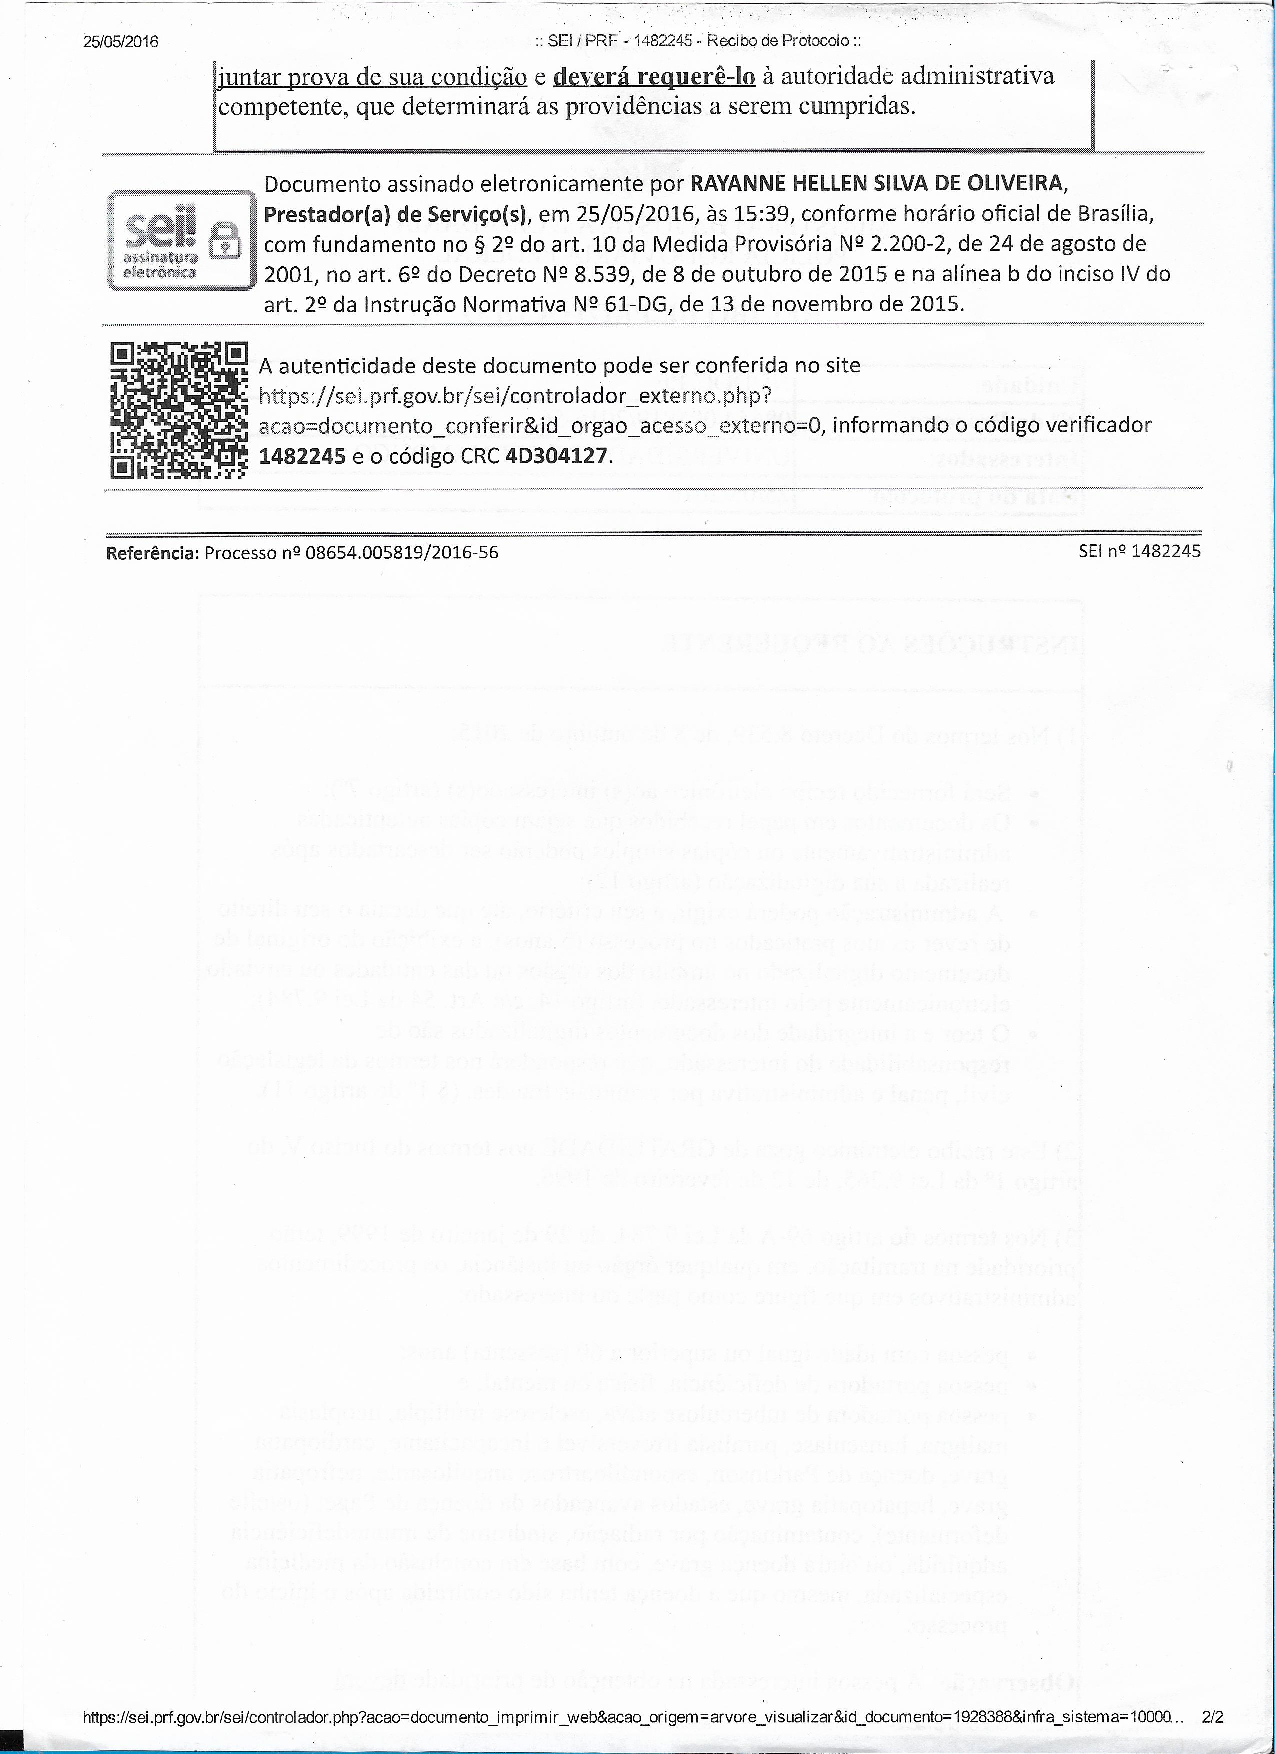
\includegraphics[scale=0.30]{Figuras/Anexos/A1-PRFDadospg_005.pdf}
		\label{fig:Documento liberação dos dados PRF}
\end{figure}

\pagebreak


\begin{figure}[ht!]
	\centering
	\caption{Documento liberação dos dados BPRv}
	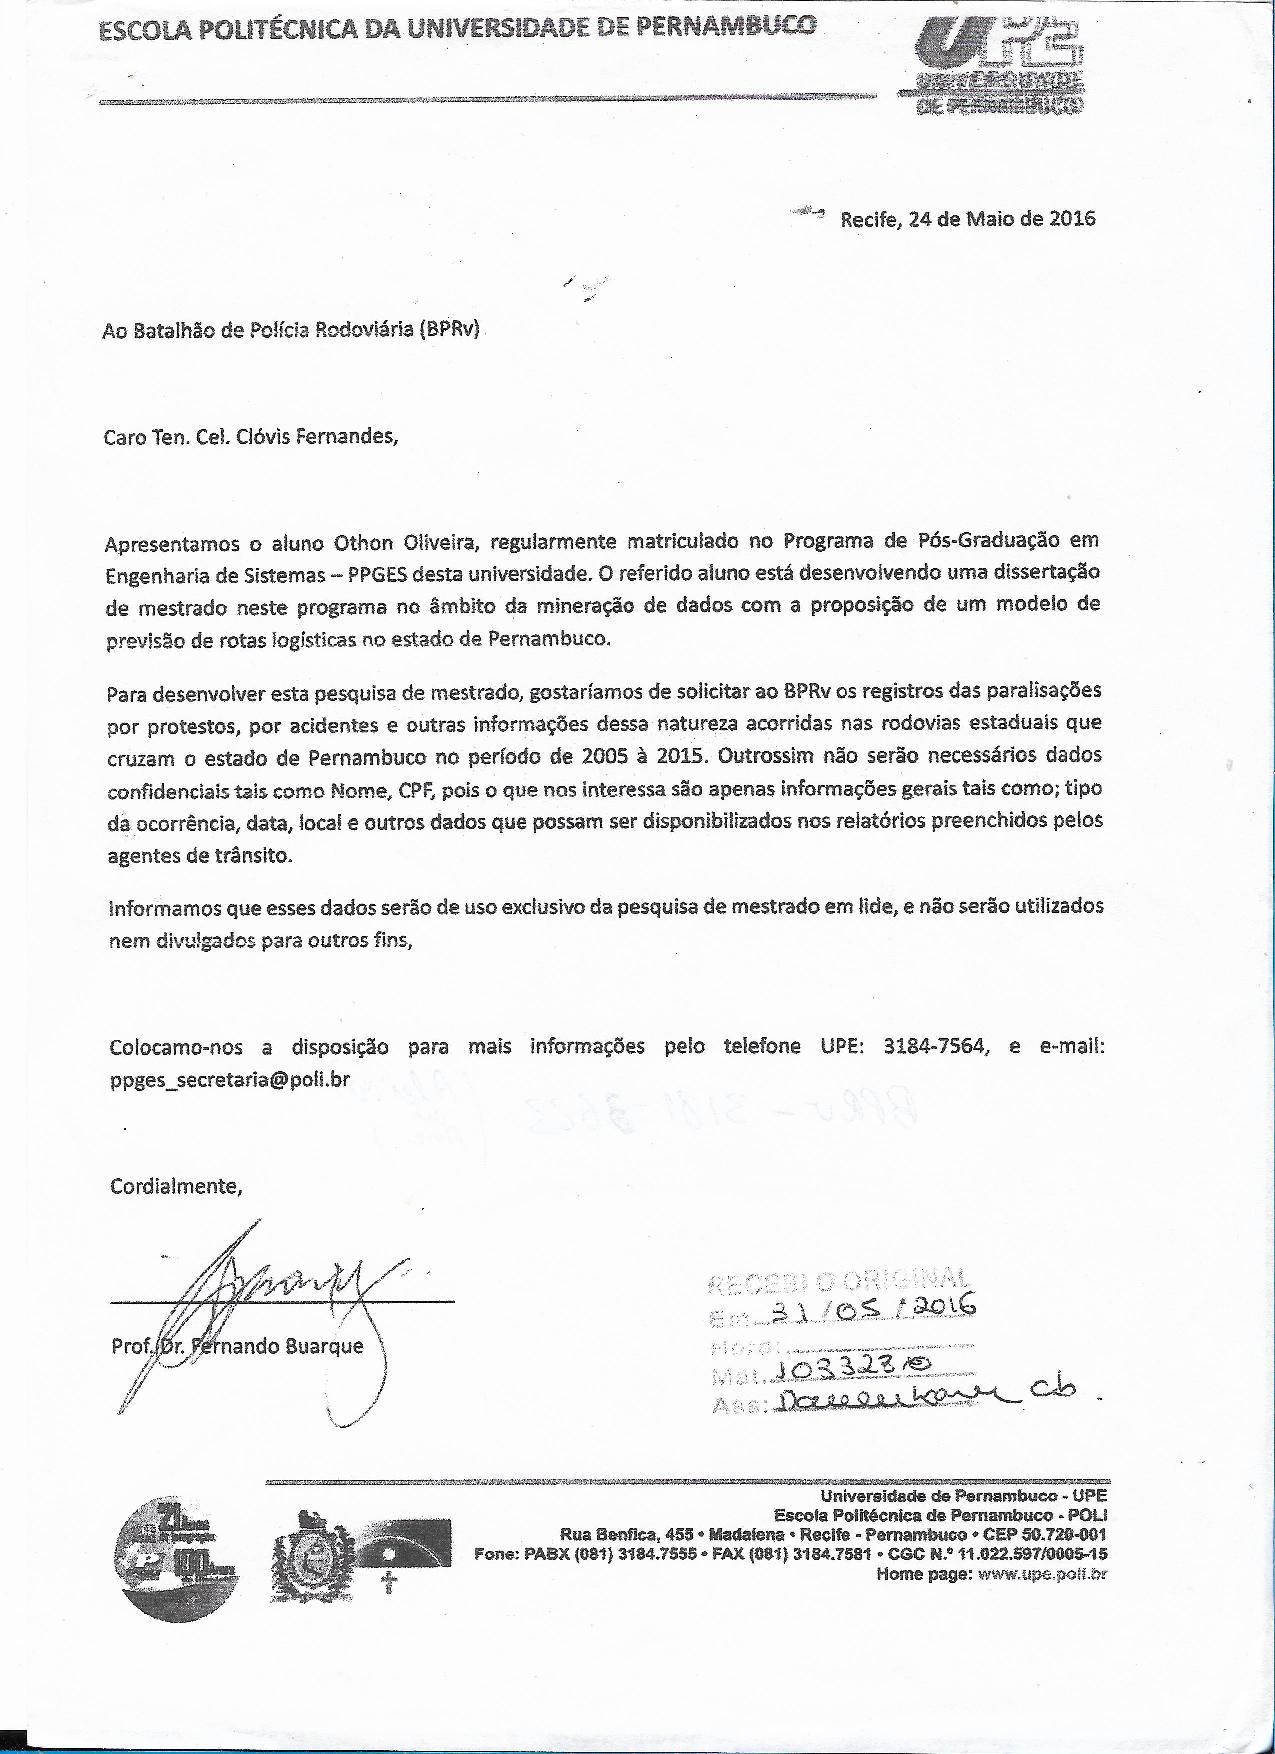
\includegraphics[scale=0.35]{Figuras/Anexos/A1-BPRvpg001.pdf}
	%\qquad \quad \quad
	%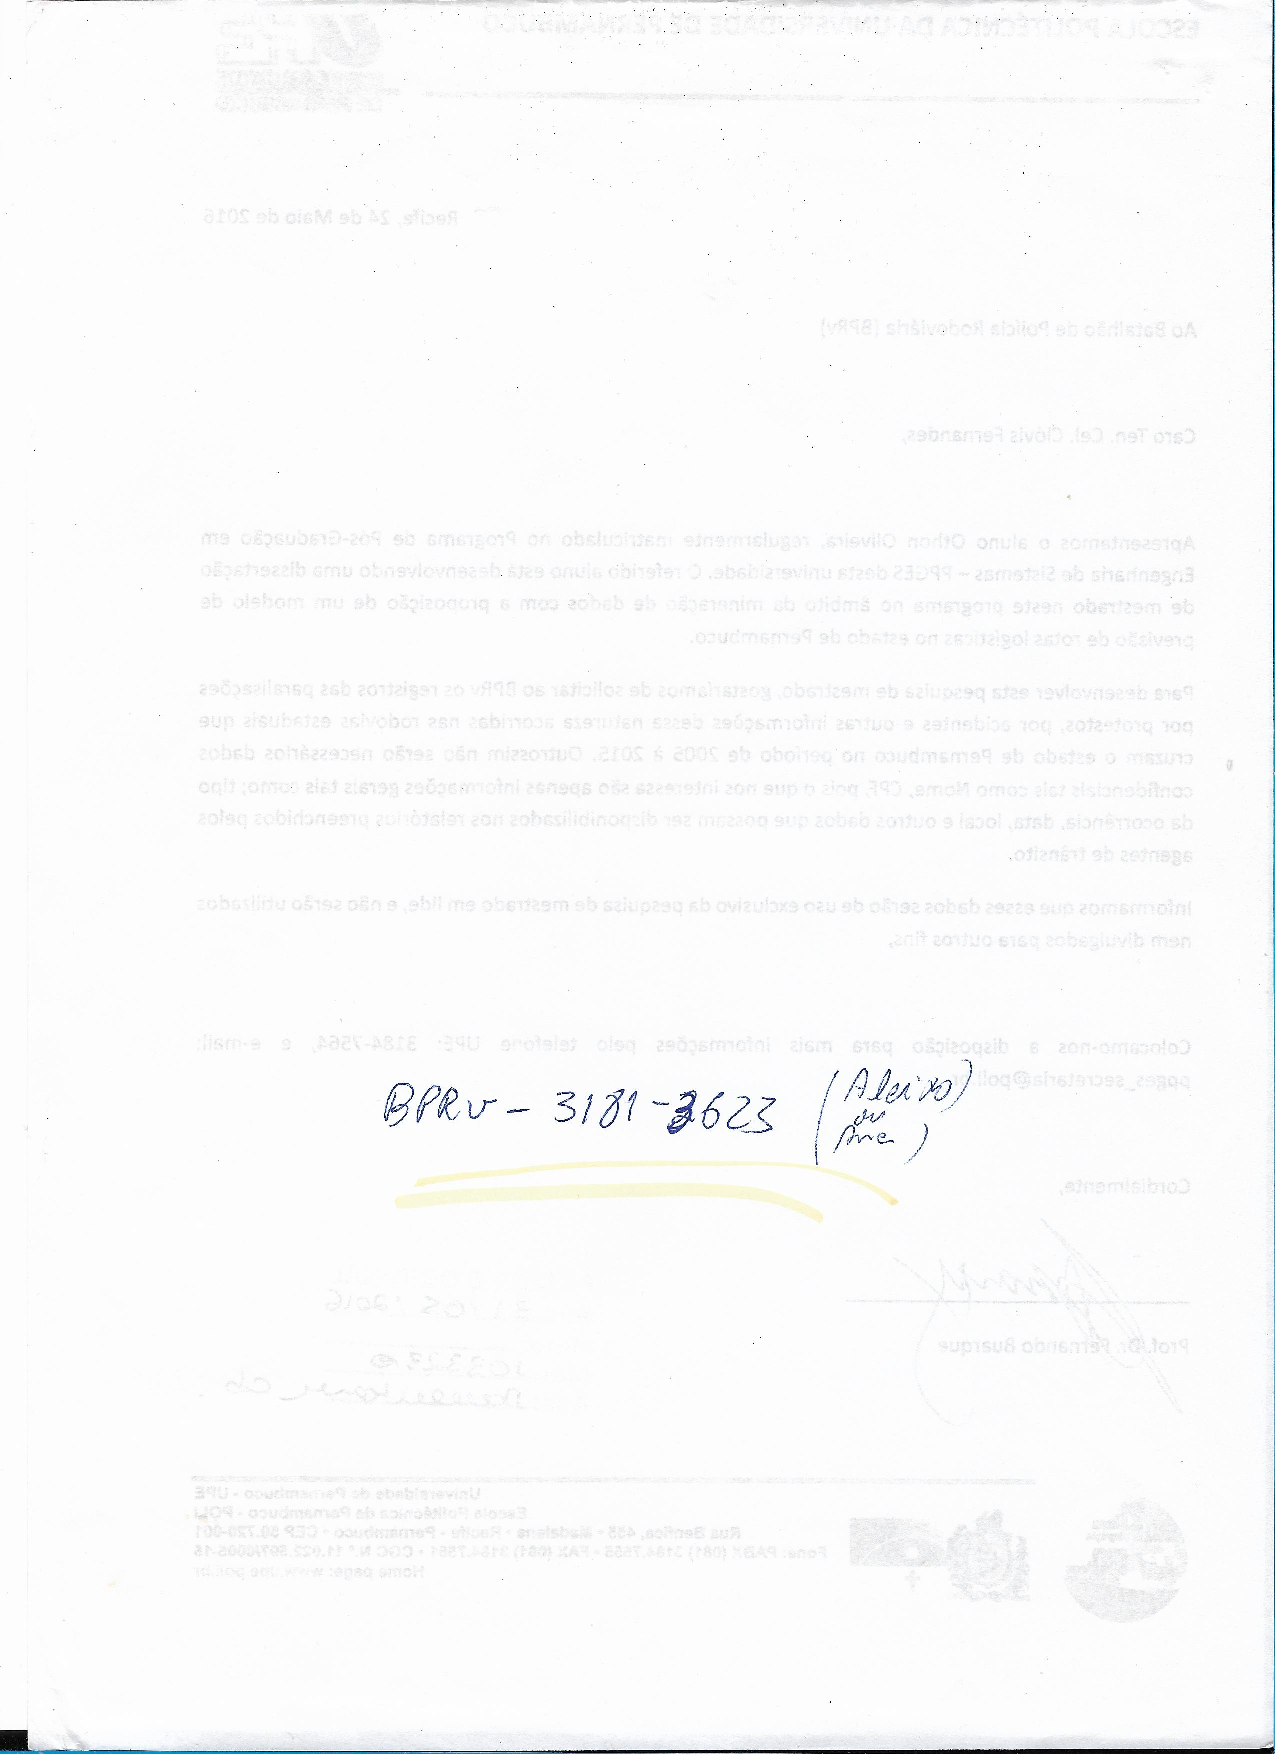
\includegraphics[scale=0.30]{Figuras/Anexos/A1-BPRvpg002.pdf}
	%\label{fig:Documento liberação dos dados PRF}
\end{figure}

\begin{figure}[ht!]
	\centering
	\caption{Frota de veículos de Pernambuco - por cidade}
	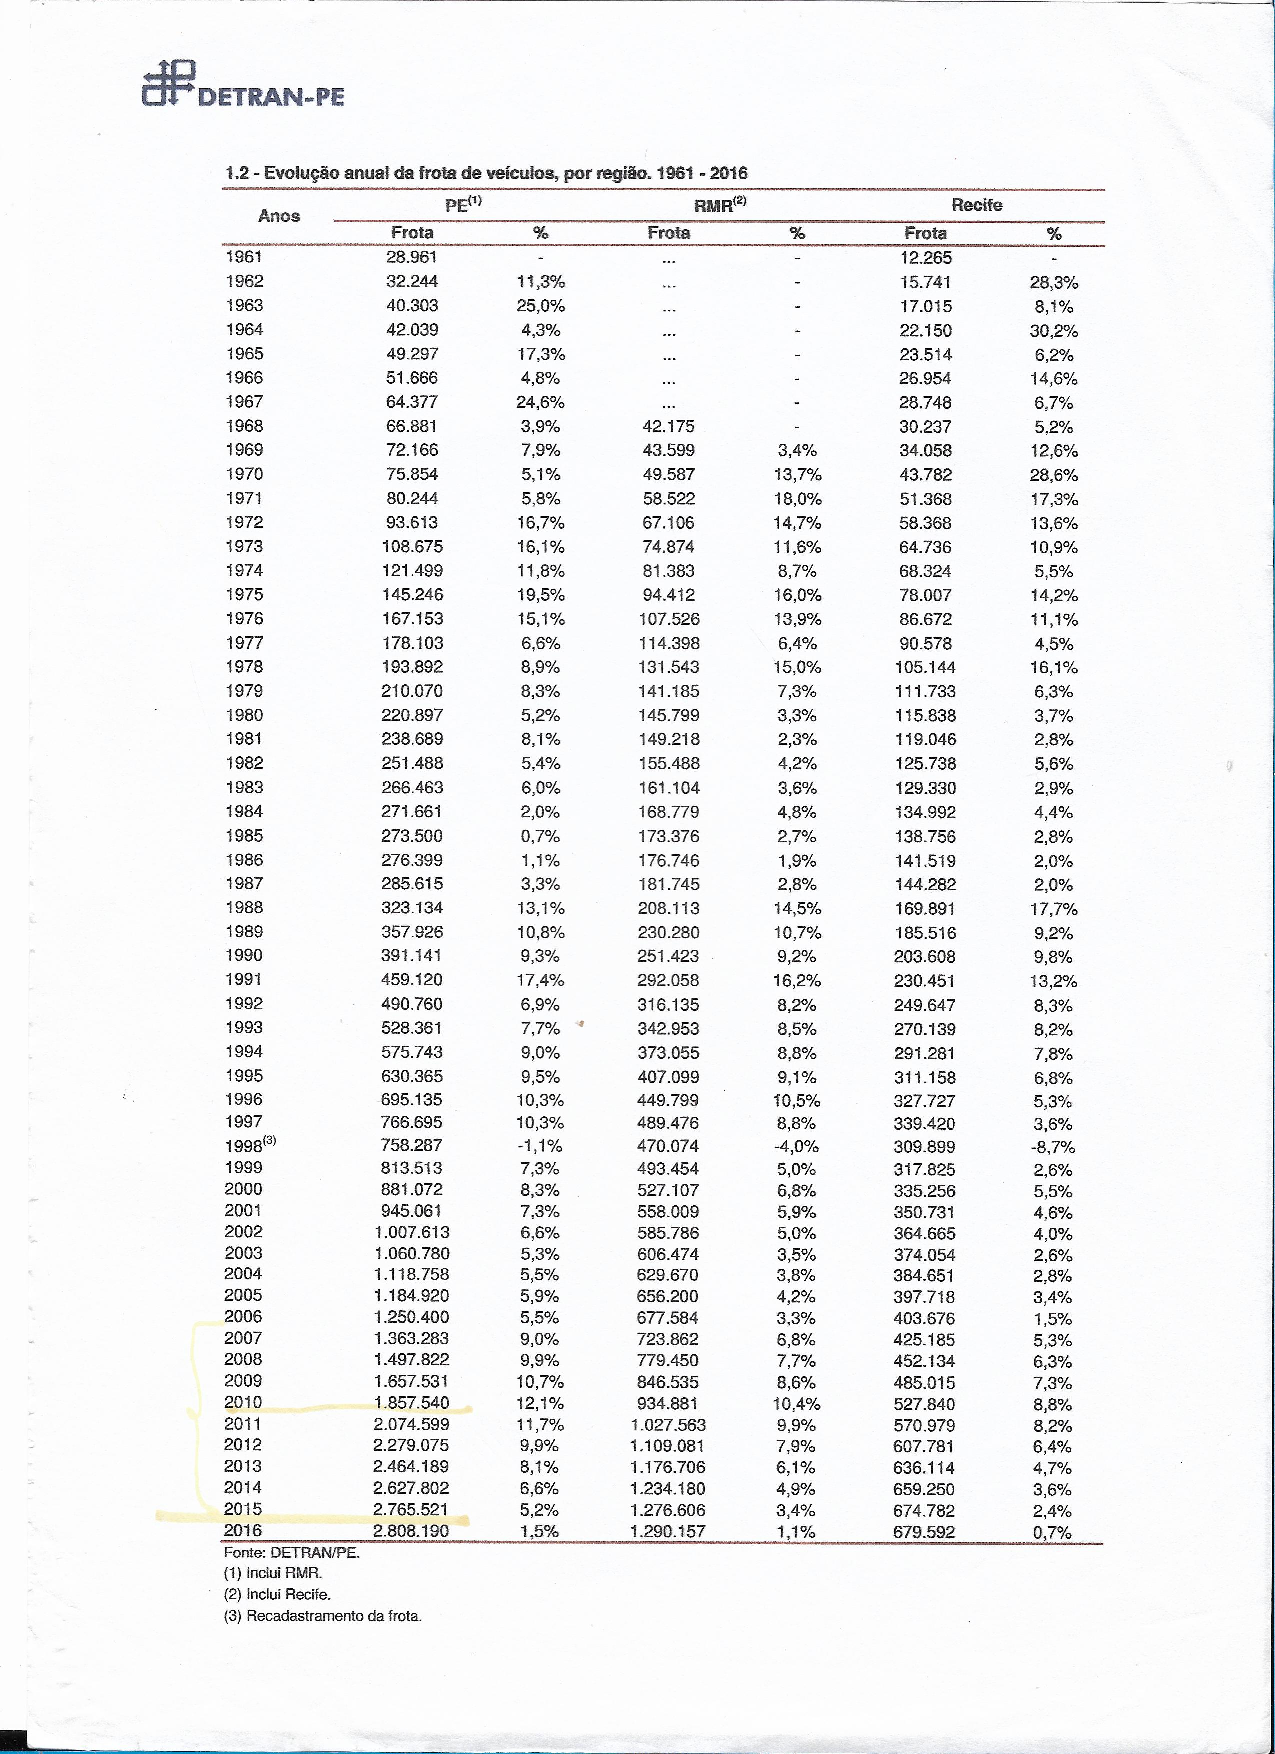
\includegraphics[scale=0.35]{Figuras/Anexos/A1-FrotaPE.pdf}
	%\qquad \quad \quad
	%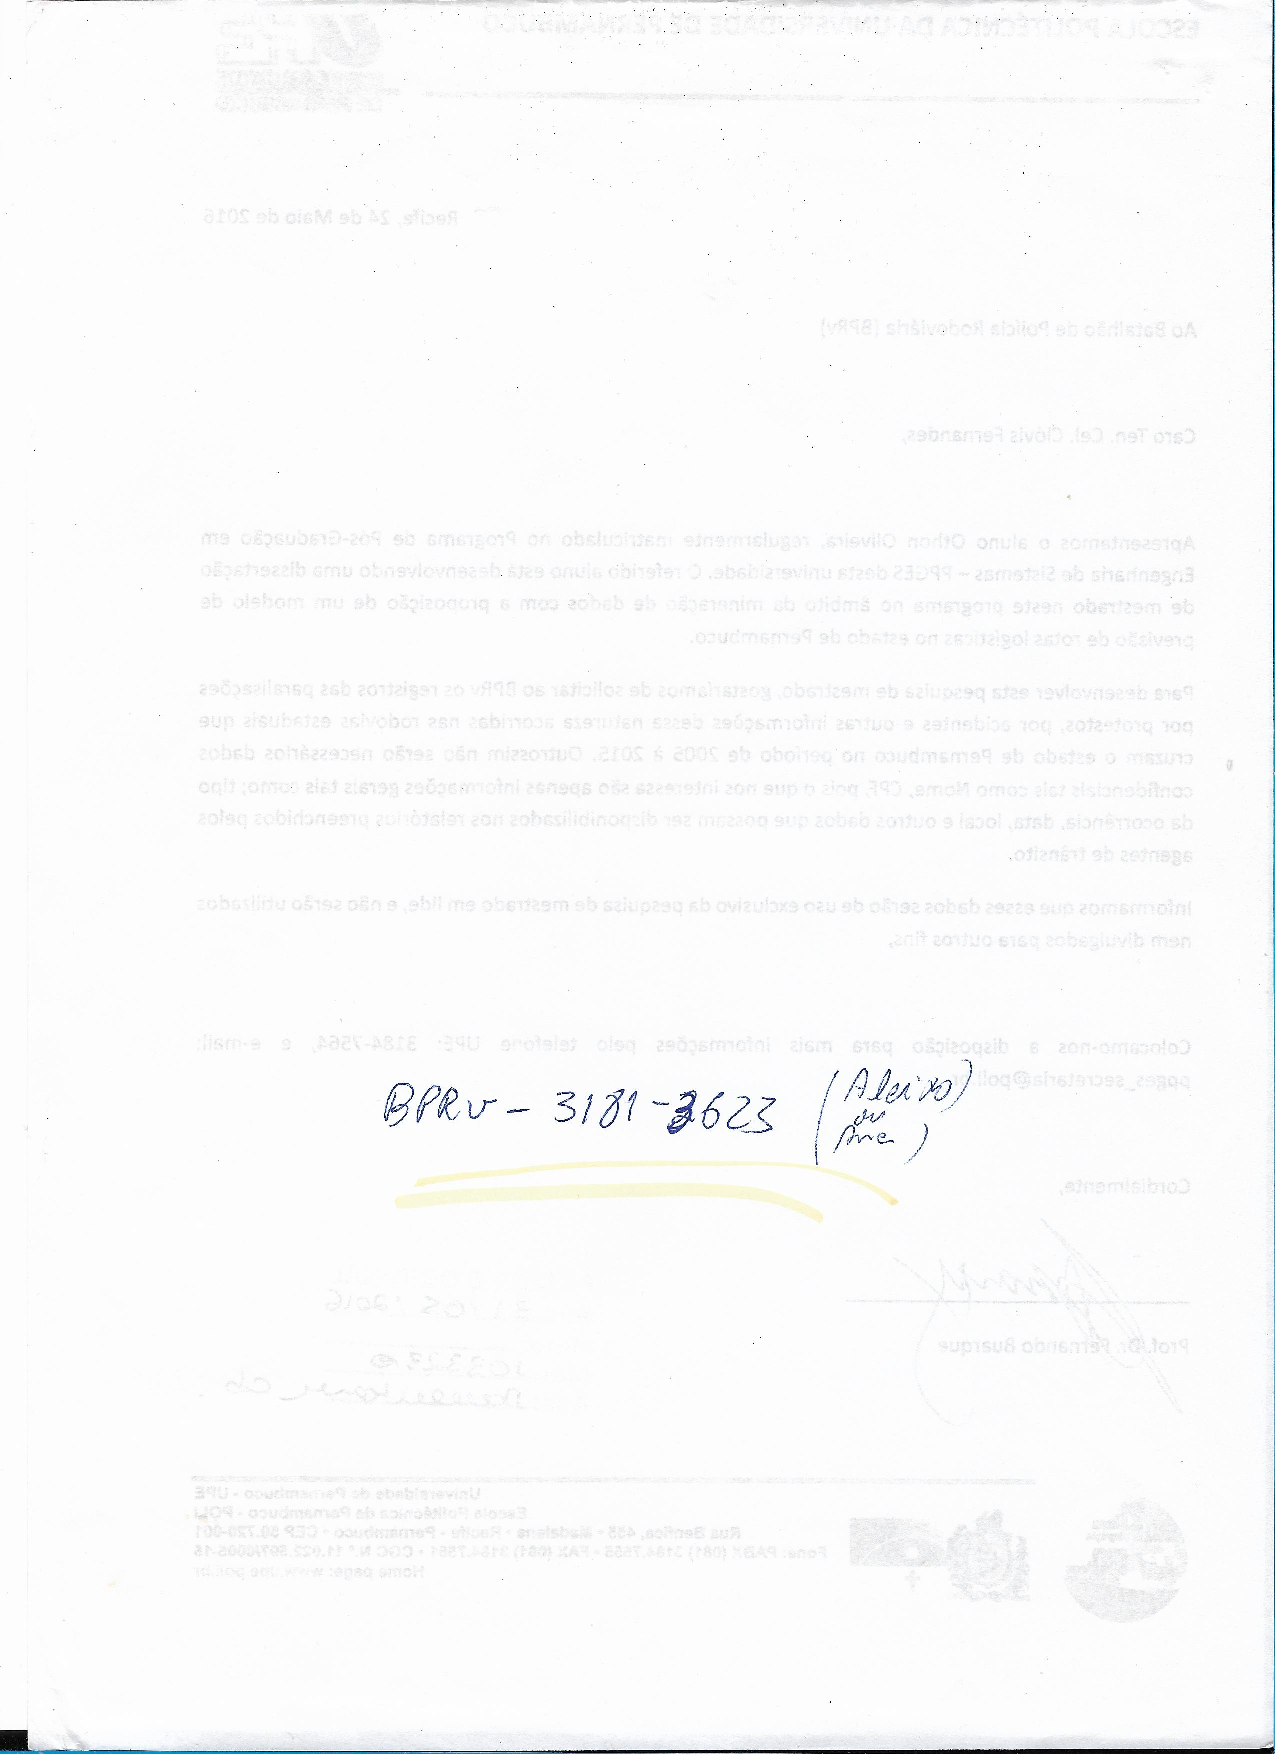
\includegraphics[scale=0.30]{Figuras/Anexos/A1-BPRvpg002.pdf}
	%\label{fig:Documento liberação dos dados PRF}
\end{figure}
	
%\pagebreak

%	\begin{figure}[ht!]
%		\centering
%		%\caption{Dados originais do Twitter}
%		\includepdf[pages=2,pagecommand={}, offset=-1.0cm -0.01cm]{Figuras/Anexos/A1-PRFDados.pdf}
%		\label{fig:Documento liberação dos dados PRF}
%	\end{figure}

		

